\section{Real-Time Defined}

\begin{frame}
   {What is Real-Time?}

   \begin{itemize}
      \item
      Correctness is not just about writing bug-free, efficient code.
      \item
      It also means \textbf{executing at the correct time}.
      \item
      And failing to meet timing restrictions leads to an error.
      \item
      This requires:
      \begin{itemize}
         \item
         deterministic runtime/scheduling behavior
         \item
         interruptibility
         \item
         priority inversion avoidance
      \end{itemize}
   \end{itemize}

\end{frame}

\cprotect\note{

   The Linux \textbf{PREEMPT\_RT} patchset helps to dramatically improve
   the real-time features of Linux. This patchset is currently
   being pushed mainline, piece by piece. Many of the pieces are
   already mainline. For example:

   \begin{itemize}
      \item generic interrupt subsystem
      \item generic timekeeping
      \item generic timer handling
      \item high resolution timers
      \item consolidation of the locking infrastructure
      \item tracing infrastructure
      \item threaded interrupt handlers
   \end{itemize}

   Various boot options and strategies will be mentioned later to help
   improve the real-time features of Linux (with or without the
   \textbf{PREEMPT\_RT} patchset).

   Visit the Linux Foundation Real-Time Wiki at:
   \url{https://wiki.linuxfoundation.org/realtime}

}

\begin{frame}
   {Priority Inversion}

   \begin{figure}[H]
      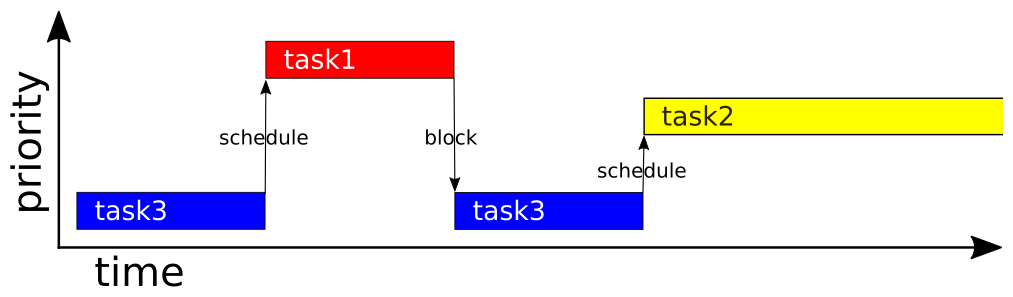
\includegraphics[width=6in]{IMAGES/priorityinversion}
      \caption{An example of priority inversion.}
   \end{figure}

   In this example, task3 is holding a lock that task1 wants. However,
   task3 never gets a chance to release that lock because it was
   interrupted by task2.

\end{frame}

\cprotect\note{

   The events leading to priority inversion:

   \begin{itemize}
      \item task3 acquires a lock
      \item task1 later tries to acquire that lock
      \item task1 blocks and task3 is scheduled so it can release the lock
      \item task2 interrupts task3 and runs unbounded
      \item task1 is now (indirectly) waiting on task2... priority inversion
   \end{itemize}

}

\begin{frame}
   {Priority Inheritance}

   \begin{figure}[H]
      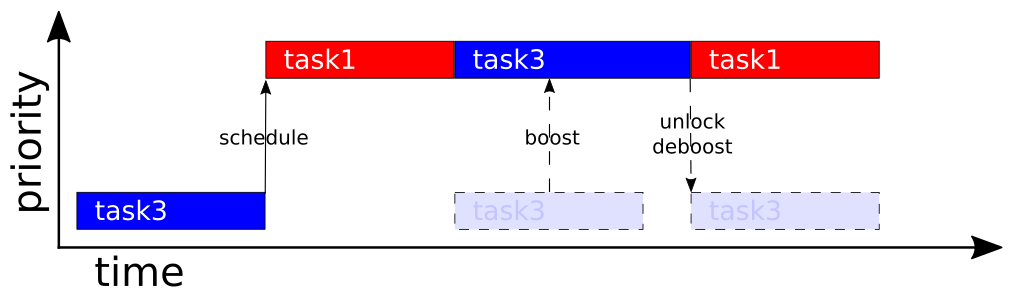
\includegraphics[width=6in]{IMAGES/priorityinheritance}
      \caption{An example showing priority inheritance.}
   \end{figure}

   Linux supports \textbf{priority inheritance} to temporarily
   boost the priority of task3 once task1 tries to acquire the
   lock. This results in task1 acquiring the lock as soon as
   possible.

\end{frame}

\cprotect\note{

   There are two common methods for avoiding priority inversion:

   \begin{itemize}
      \item \textbf{priority inheritance}: When a task of higher
            priority wants a resource held by a task of lesser
            priority, the priority of the resource holder is
            "boosted" to that of the higher priority task until
            that resource is made available.
      \item \textbf{priority ceiling}: Instead of assigning
            priorities to tasks, priorities are assigned to
            resources. When any task acquires a resource, it
            is assigned the priority of that resource until it
            is released.
   \end{itemize}

}
